%--------------------------------------------------------------------------------------------------
\chapter{Einbinden des Menschmodells und Validierung der Anforderungen}\label{cha:ValidierungDesKonzepts}
In diesem Kapitel wird zunächst die Vorgehensweise für das Einbinden des Menschmodells in ein neues Projekt und das Einfügen neuer Objekte in der Umgebung erklärt. Daraufhin wird erläutert, warum die in Kapitel \ref{sec:AnforderungenKonzept} gestellten Anforderungen an das Menschmodell und an die Interaktionsschnittstelle gewährleistet werden.

%--------------------------------------------------------------------------------------------------
\section{Einbinden des Menschmodells in ein neues Projekt}\label{sec:MenschmodellEinbinden}
Um das Einbinden des Menschmodells in ein beliebiges Projekt einfach zu gestalten, gibt es in diesem Abschnitt eine Erläuterung der Vorgehensweise. Dabei sind die folgenden drei Schritte zu befolgen: Vorbereitung der Entwicklungsumgebung, Einfügen der Vorlage in das neue Projekt und Einfügen in die Szene.

\subsection{Schritt 1: Vorbereitung der Entwicklungsumgebung}
Im ersten Schritt muss die Entwicklungsumgebung vorbereitet werden. Dafür muss zunächst mit Hilfe der in Kapitel XX erläuterten Programme VIVE Wireless und SteamVR eine Verbindung mit der VR Hardware ermöglicht werden. Es ist zu empfehlen, die aktuellsten Versionen dieser Programme zu nutzen. Des Weiteren muss die Unity Entwicklungsumgebung installiert werden. Dabei ist zu beachten, dass diese Arbeit, wie bereits in Kapitel XX erwähnt, auf Grundlage der Version 2019.2.19f1 von Unity entwickelt wurde. Schließlich müssen noch die in Kapitel XX erläuterten Plugins SteamVR und Final IK aus dem Asset Store heruntergeladen und in dem aktuellen Projekt importiert werden.

\subsection{Schritt 2: Einfügen der Vorlagen in das neue Projekt}
Im zweiten Schritt müssen die Vorlagen des Menschmodells in das neue Projekt eingefügt werden. Es ist ausreichend, die in Kapitel \ref{fig:UnityOverview} dargestellten Ordner 'Prefab', 'Scenes' und 'Scripts' zu kopieren und in das Verzeichnis des neuen Projekts einzufügen. Dabei ist anzumerken, dass ein Prefab in Unity eine Objektvorlage darstellt, die beliebig oft instanziiert werden kann, daher befinden sich im Ordner 'Prefab' sämtliche Objektvorlagen des Projekts. In dem Ordner 'Scenes' befinden sich drei Demo-Szenen, unter anderem auch die in Abbildung \ref{fig:UnityOverview} dargestellte Szene und im Ordner 'Scripts' befinden sich sämtliche Skripte des Projekts. Eine genauere Erläuterung der Ordnerstruktur folgt im weiteren Verlauf dieses Kapitels.

\subsection{Schritt 3: Einfügen in die Szene}
Im letzten Schritt muss lediglich das Menschmodell in die Szene eingefügt werden. Dabei steht dem Entwickler frei, ob das Menschmodell, die Interaktionsschnittstelle oder beides zusammen in das neue Projekt eingebunden werden soll. Um das Menschmodell in das neue Projekt einzubinden, muss lediglich das Prefab 'Human' eingefügt werden, während bei der Interaktionsschnittstelle neben dem Prefab 'InteractionEventSystemAndScripts' noch das SteamVR CameraRig in der Szene eingefügt werden muss. Falls das Menschmodell in Kombination mit der Interaktionsschnittstelle verwendet werden soll, ist es ausreichend wie in Abbildung \ref{fig:UnityOverview} dargestellt, einfach das Prefab 'Human+Interaction' in der Szene zu platzieren.

\section{Vorgehensweise beim hinzufügen neuer Objekte in die Szene}\label{sec:ObjekteEinbinden}
Genauso wie das Menschmodell inklusive der Interaktionsschnittstelle können beliebige Objekte ohne großen Aufwand in das Unity Projekt integriert werden. Dabei sind die folgenden drei Schritte zu befolgen: Einfügen in die Ordnerstruktur des Projekts, Einfügen in die Szene und Einbinden in die Menüs.

\subsection{Schritt 1: Einfügen in die Ordnerstruktur des Projekts}
\begin{figure}[h]
	\centering
	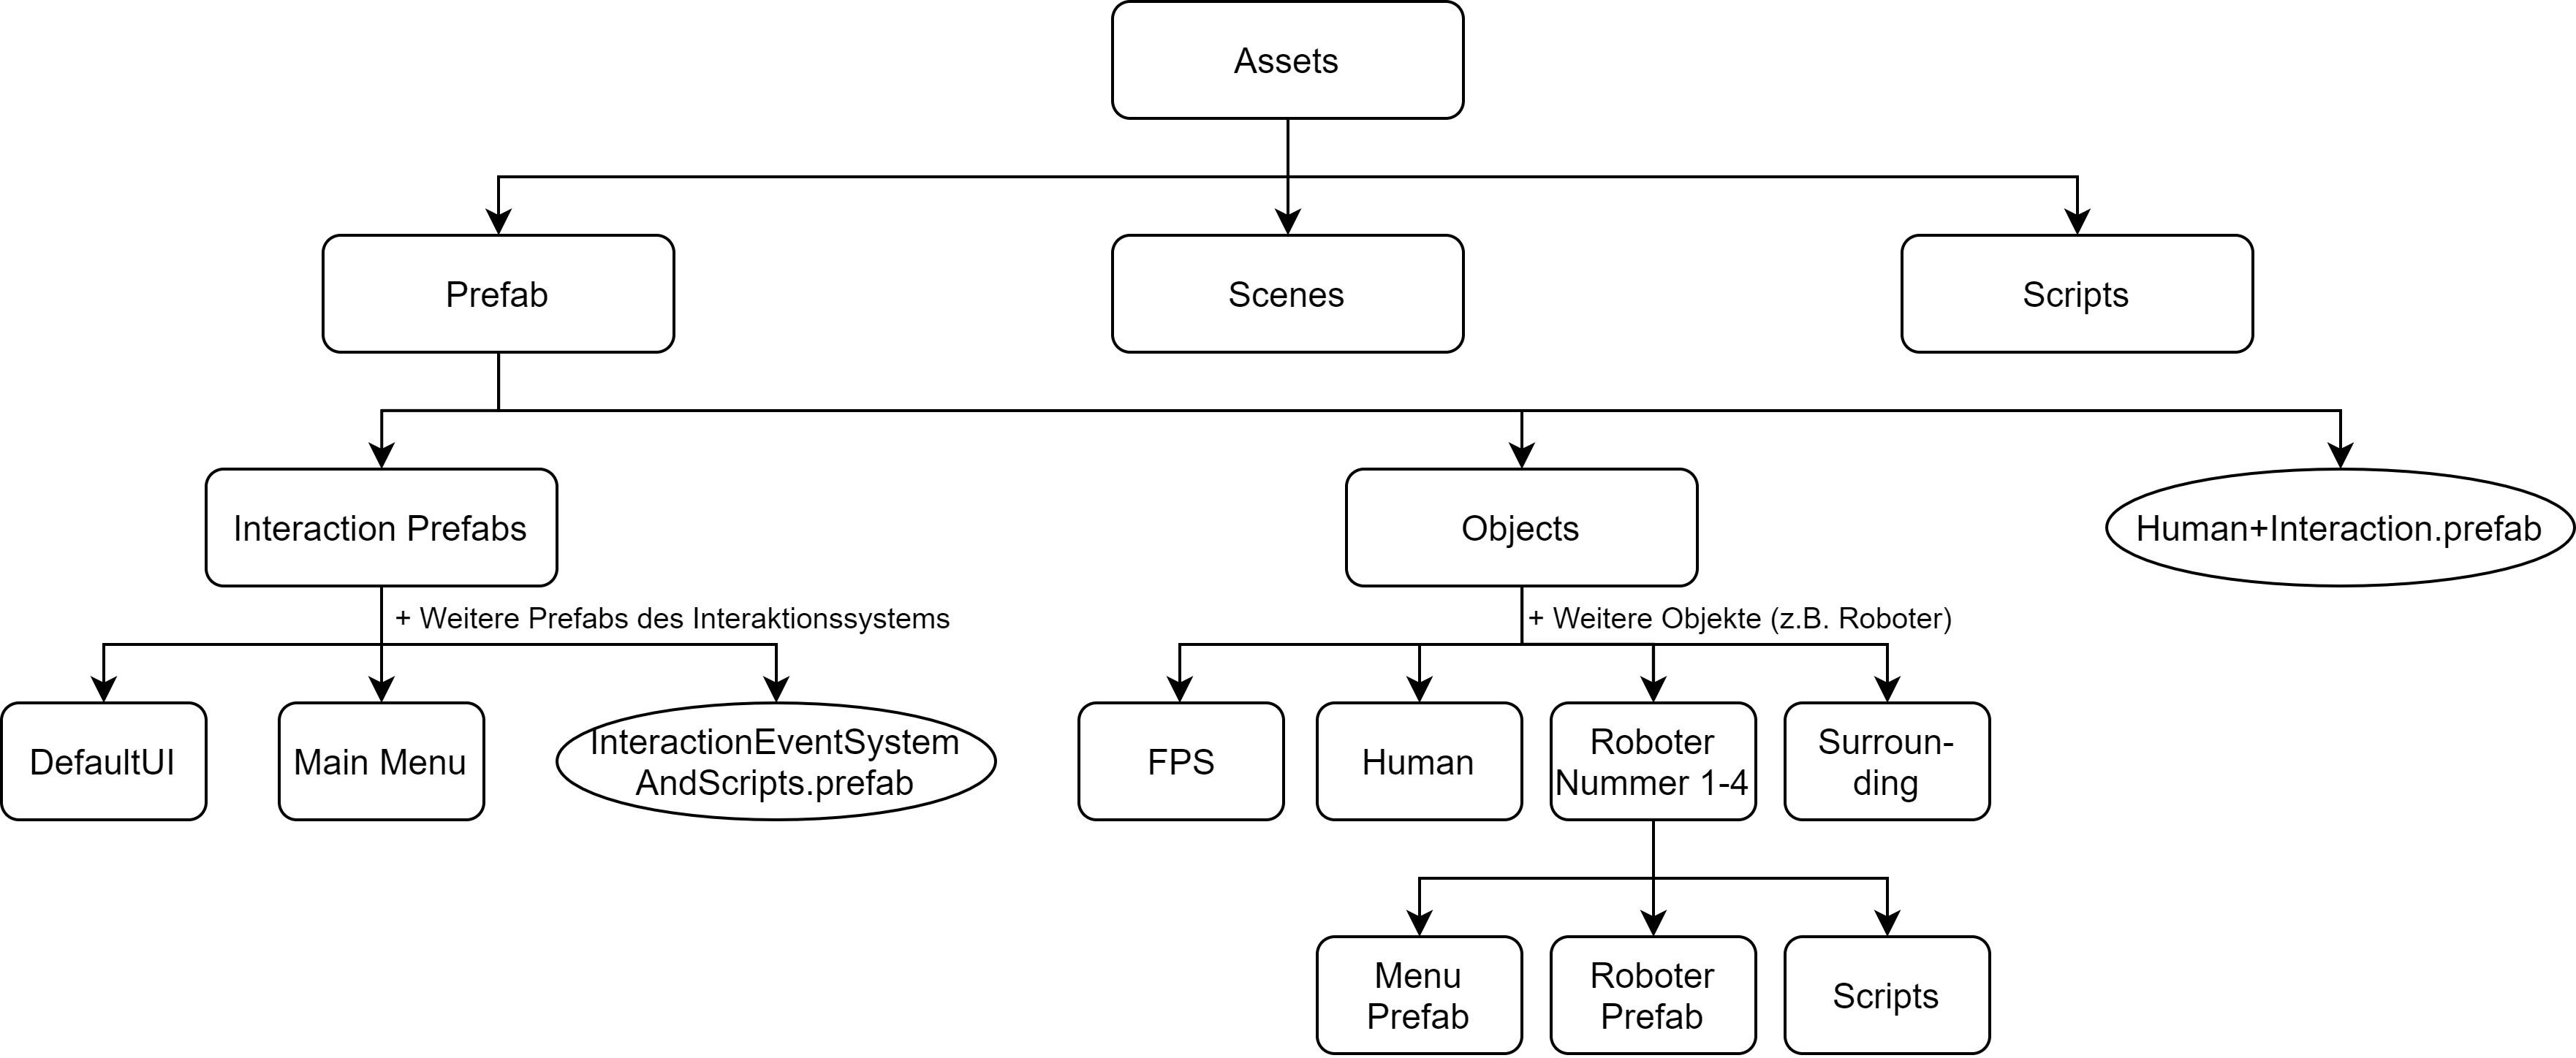
\includegraphics[width=1\linewidth]{Bilder/A54_Ordnerstruktur}
	\caption{Die Ordnerstruktur, eigene Abbildung}
	\label{fig:Ordnerstruktur}
\end{figure}
\noindent Bevor erklärt wird, wie neue Objekte in das Projekt eingefügt werden, gibt es zunächst eine Einführung in den Aufbau der Ordnerstruktur des Projekts. In der Abbildung \ref{fig:Ordnerstruktur} sind die wichtigsten Ordner des Projekts abgebildet. Es ist anzumerken, dass Ordner durch Rechtecke und Objekte durch Ovale abgebildet werden.
\newline\newline
Auf der obersten Ebene befinden sich die Ordner \textbf{'Prefab'}, \textbf{'Scenes'} und \textbf{'Scripts'}. In dem Ordner 'Scenes' sind wie bereits erwähnt die drei Demo-Szenen und in dem Ordner 'Scripts' die Skripte abgespeichert. Neben den vorhandenen Demo-Szenen empfiehlt es sich in Zukunft alle weiteren Szenen in diesem Ordner abzuspeichern. Im Gegensatz dazu sollte der Inhalt des Ordners 'Scripts' größtenteils unverändert bleiben, da sich in diesem Ordner lediglich die Skripte für das Menschmodell und die Interaktionsschnittstelle verändern. Lediglich die Skripte Spawning Handler und Global Variables, die sich in einem Unterordner befinden, sollten angepasst werden, falls neue Objekte in die Umgebung eingefügt werden. Des Weiteren ist anzumerken, dass sich neben diesen drei Ordnern noch weitere Ordner auf dieser Ebene im Projekt befinden. Diese sind aber, wie z.B. in Abbildung \ref{fig:UnityOverview} zu erkennen ist, automatisch generierte Ordner die durch das Importieren der Plugins Final IK und SteamVR entstehen. 
\newline\newline
Wie bereits erwähnt, ist der Inhalt der Ordner 'Scenes' und 'Scripts' bereits bekannt. Aufgrund dessen sind in Abbildungen \ref{fig:Ordnerstruktur} des Ordners 'Prefab' abgebildet.
--> TODO erklären

\subsection{Schritt 2: Einfügen in die Szene}
--> PointerEvent Object + Collider + Platzieren

\subsection{Schritt 3: Einbinden in die Menüs}
--> Wie bereits erwähnt das mit den 2 skripten
--> Es empfiehlt sich diese neu zu schreiben, da diese wie bereits erwähnt nur zu demo zwecken erstellt wurden
--> Auch das mit falko hier

%--------------------------------------------------------------------------------------------------
\section{Validierung des Anforderungen des Menschmodells}\label{sec:ValidMensch}

\subsection{Anforderung 1: Genauigkeit}
Durch die Möglichkeit, die Bewegungen des Bedieners an bis zu zehn Körperteilen (Beide Füße, beide Knie, Steißbein, beide Hände, beide Ellenbogen und Kopf) zu verfolgen und diese Daten bei der Abbildung auf den virtuellen Menschen zu berücksichtigen, wird die in Kapitel \ref{sec:AnforderungenKonzept} geforderte Genauigkeit erfüllt. Zusätzlich wird die Genauigkeit, durch die Möglichkeit das Menschmodell zu Kalibrieren, also an die Körpergröße des Bedieners anzupassen, verbessert. So könnte man in Zukunft für jeden beliebigen Bediener mit Hilfe des Menschmodells einen virtuellen Klon für die virtuelle Welt schaffen, in dem man die Textur für den in Kapitel \ref{sec:MMModell} angesprochenen Skinned Mesh Renderer anpasst.

\subsection{Anforderung 2: Echtzeit}
Mit Hilfe des Plugins Final IK werden die Bewegungsdaten des Bedieners in nahezu Echtzeit verarbeitet und auf das Menschmodell übertragen. Es sind keine sichtbaren Verzögerungen zu erkennen, die die Nützlichkeit des Menschmodells einschränken würden oder sogar eine potenzielle Gefahrenquelle darstellen könnten. Aufgrund dessen wird die in Kapitel \ref{sec:AnforderungenKonzept} gestellte Anforderung an die Echtzeit ebenfalls erfüllt.

\subsection{Anforderung 3: Interoperabilität}
Das Menschmodell wurde umgebungsunabhängig implementiert, ist also von keinen anderen Komponenten der virtuellen Umgebung abhängig. Folglich kann das Menschmodell in jeder beliebigen virtuellen Umgebung, wie Beispielsweise virtuell begehbare Produktionsanlagen, eingesetzt werden und erfüllt somit die in Kapitel \ref{sec:AnforderungenKonzept} gestellte Anforderung an die Interoperabilität.

\subsection{Anforderung 4: Modularität}
Wie in Abbildung \ref{fig:UnityOverview} zu erkennen ist, ist das Menschmodell modular aufgebaut und erlaubt einfache Anpassungen und Erweiterungen in der Zukunft. Insgesamt besteht das Menschmodell (ohne die Interaktionsschnittstelle) aus den vier Komponenten Kamera, Modell, Skripte und Verfolgungsziele, welche selber nochmal aus einigen Komponenten bestehen. Aufgrund dessen wird die in Kapitel \ref{sec:AnforderungenKonzept} geforderte Modularität gewährleistet.

%--------------------------------------------------------------------------------------------------
\section{Validierung der Anforderungen der Interaktionsschnittstelle}\label{sec:ValidInteraktion}

\subsection{Anforderung 1: Bidirektionalität}
Der Informationsaustausch zwischen Mensch und Maschine findet bidirektional statt, da der Mensch durch den Pointer die Möglichkeit erhält über graphische Benutzeroberflächen mit der Maschine zu interagieren. In anderen Worten stellt der Pointer das Input-Medium des Menschen dar. Gleichzeitig ermöglichen die graphischen Benutzeroberflächen die Darstellung von Feedback der Produktionsanlagen. So könnten Beispielsweise Produktionsraten, Stromverbrauch oder sonstige produktionstechnisch relevante Parameter angezeigt werden. Aufgrund dessen wird die in Kapitel \ref{sec:AnforderungenKonzept} geforderte Anforderung der Bidirektionalität erfüllt.

\subsection{Anforderung 2: Genauigkeit}
Mit Hilfe des Pointers, der durch das Bewegen der rechten Hand gesteuert wird, wird ein sehr präzises und vor allem intuitives interagieren mit der Umgebung ermöglicht. Aufgrund dessen wird die in Kapitel \ref{sec:AnforderungenKonzept} geforderte Genauigkeit bei der Interaktion mit der Umgebung gewährleistet.

\subsection{Anforderung 3: Echtzeit}
Durch die Verarbeitung der Bewegungsdaten in Echtzeit wird nicht nur die nahezu verzögerungslose Abbildung des Menschmodells, sondern auch eine nahezu verzögerungslose Interaktion mit der Umgebung ermöglicht. Dies ermöglicht den Bedienern schnell auf Veränderungen in der virtuellen Umgebung zu reagieren und spontane Anpassungen zu tätigen. Aufgrund dessen wird die in Kapitel \ref{sec:AnforderungenKonzept} gestellte Anforderung an die Echtzeit ebenfalls erfüllt.

\subsection{Anforderung 4: Interoperabilität}
Die Interaktionsschnittstelle ist, bis auf wenige Skripte und dem Interaktionssystem, nicht von der Umgebung abhängig. Daher ist es ausreichend, die eben angesprochenen Komponenten irgendwo in der Szene zu hinterlegen (Vgl. Abbildung \ref{fig:UnityOverview}). Um eine Interaktion mit beliebigen Objekten in der Szene zu ermöglichen, müssen diese lediglich mit dem Object Menu Skript und einem Collider erweitert werden. Des Weiteren müssen ihre Menüs mit Hilfe der bereits in Unity vorhanden Komponenten für graphische Benutzeroberflächen implementiert sein. Folglich wird die in Kapitel \ref{sec:AnforderungenKonzept} geforderte Interoperabilität gewährleistet, da sich die beschrieben Funktionalität auf beliebige Objekte übertragen lässt, solange die entsprechenden Rahmenbedingungen eingehalten werden.

\subsection{Anforderung 5: Modularität}
Sowohl das Menschmodell, als auch die Interaktionsschnittstelle sind Modular aufgebaut und bestehe aus austauschbaren Komponenten. Es ist beispielsweise möglich, die Interaktionsschnittstelle für andere VR Hardware einsatzfähig zu machen. Dafür müssen lediglich die entsprechenden Input Schnittstellen der VR Hardware in einigen Skripten angepasst werden. Des Weiteren wurden das Menschmodell und die Interaktionsschnittstelle getrennt voneinander entwickelt, um die Unabhängigkeit und somit die in Kapitel \ref{sec:AnforderungenKonzept} geforderte Modularität zu gewährleisten.

%--------------------------------------------------------------------------------------------------